
\subsection{Application to the test vehicle}

The method described in both previous sections (\ref{sec:block-failure-cz} and \ref{sec:block-chaining}) is tested in simulation on real blocks.
More precisely, it will be tested against the regulation function of the testchip.

% Which pins are selected for characterization
This function is composed of three blocks, a pre-regulator, a bandgap and a regulator.
For each one, an input and output pin are selected.
The input/outputs that play a key role on the regulation function were selected on the regulation function.
Details of the selected pins is given in Table \ref{selected-pins-for-cz}.

\begin{table}[]
\centering
\begin{tabularx}{\linewidth}@{}|c|c|c|c|c|c|c|@{}}
\toprule
{ \textbf{IC block}} & { \textbf{input pin}}                 & \multicolumn{1}{l|}{{ }} & { }                                & \multicolumn{1}{l|}{{ }}               & { \textbf{output pin}}            & { }                          \\ \midrule
{ }                  & { \textbf{specification}}             & { \textbf{DC value (V)}} & { \textbf{stress amplitude range}} & { \textbf{stress width range}}         & { \textbf{specification}}         & { \textbf{Failure criteria}} \\ \midrule
{ pre-regulator}     & { external supply battery connection} & { 12V}                   & { -1V to -10V with 1V step}        & { 1ns to 1000ns with 30 pts log scale} & { 9V clamped voltage}             & { vclamp9 \textless 0V}      \\ \midrule
{ bandgap}           & { 9V clamped voltage}                 & { 9V}                    & { -1V to -15V with 1V step}        & { 1ns to 1000ns with 30 pts log scale} & { bandgap voltage 2.5V reference} & { vref2p5 \textless 1.25V}   \\ \midrule
{ regulator}         & { bandgap 2.5V reference}             & { 2.5V}                  & { -0.5 to -10V with 0.5V step}     & { 1ns to 1000ns with 30 pts log scale} & { regulated 2.5V 20mA capability} & { v2p5 \textless 2.1 V}      \\ \bottomrule
\end{tabularx}
\caption{Selected pins for characterization and characterization limits}
\label{selected-pins-for-cz}
\end{table}

% Talk about the characterization limits and failure criteria chosen
%TODO: Detail how were chosen failure criteria
The characterization is done using negative voltages.
The goal is to exploit the weakness of the testchip against negative pulses discovered and highlighted in section \ref{sec:testchip_study}.
Basically, it was observed for sufficiently high negative voltage that a short pulse can cause a full restart of the system.
The time taken by this restart, observed on the regulator output, is several order of magnitudes longer than the original pulse injected on the pre-regulator input.
The failure criteria for the pre-regulator corresponds to XXX ?
The failure criteria for the bandgap output voltage is the DC specification ?
Finally, the failure criteria for the regulator, and thus for the complete function, corresponds to the DC specification of this function.

% Which load value for characterization
The test setup described in section \ref{sec:block-failure-cz} requires a characterization load to simulate the impact of neighbor blocks.
In a first time, a very simplistic model is employed for this load.
An arbitrary load value of 1M\textgreek{Omega}\ is initially chosen, just to perform a preliminary test.
%TODO: DETAIL MORE ?

% Simulation process
For each block, the characterization testbench is setup and a set of simulations is run.
This set is calculated with the characterization range given in Table \ref{selected-pins-for-cz}.
This type of parameterized simulations can be efficiently distributed on multiple machines.
This way, the complete characterization of a block does not take longer than the time taken by a single simulation.
Once all simulations are run, the results are analysed and plotted using the method detailed in the previous sections.

% Talk about the output
These characterization curves are given in Figs. \ref{pre_regu_wb}, \ref{bandgap_wb} and \ref{regu_wb}.
For the given testchip, it was found that the regulation function shows clear failure when exposed to negative stresses.
For simplicity, the voltage scale was simply reversed, but this doesn't affect the results in any case.

\begin{figure}[!htbp]
  \centering
  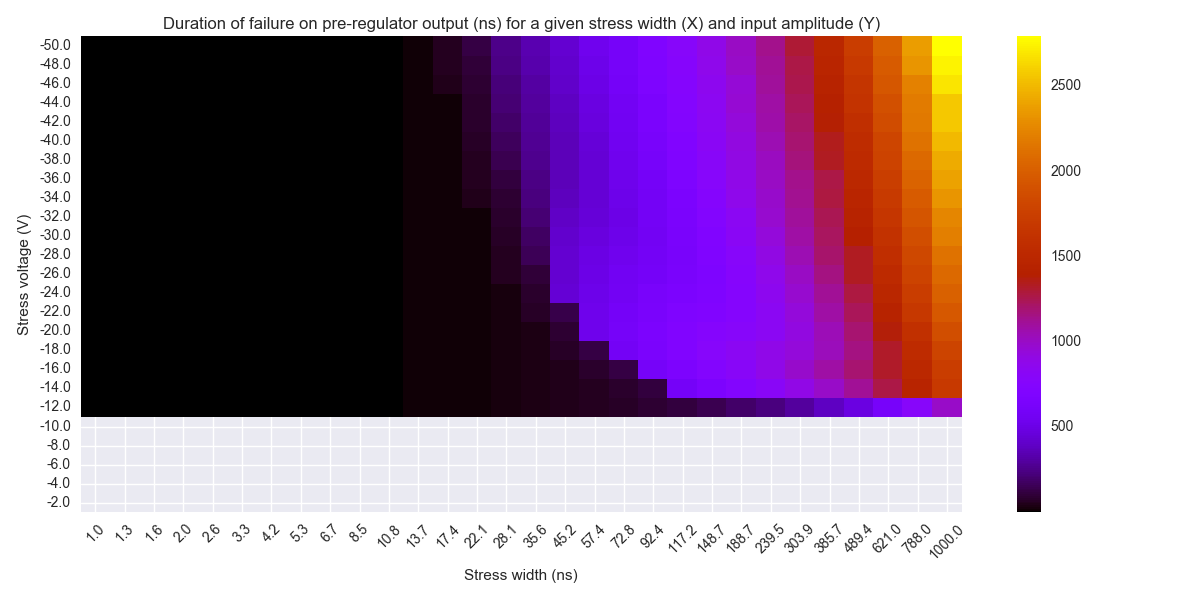
\includegraphics[width=\textwidth]{src/4/figures/preregulator_cz.png}
  \caption{Pre-regulator characterization}
  \label{pre_regu_wb}
\end{figure}

\begin{figure}[!htbp]
  \centering
  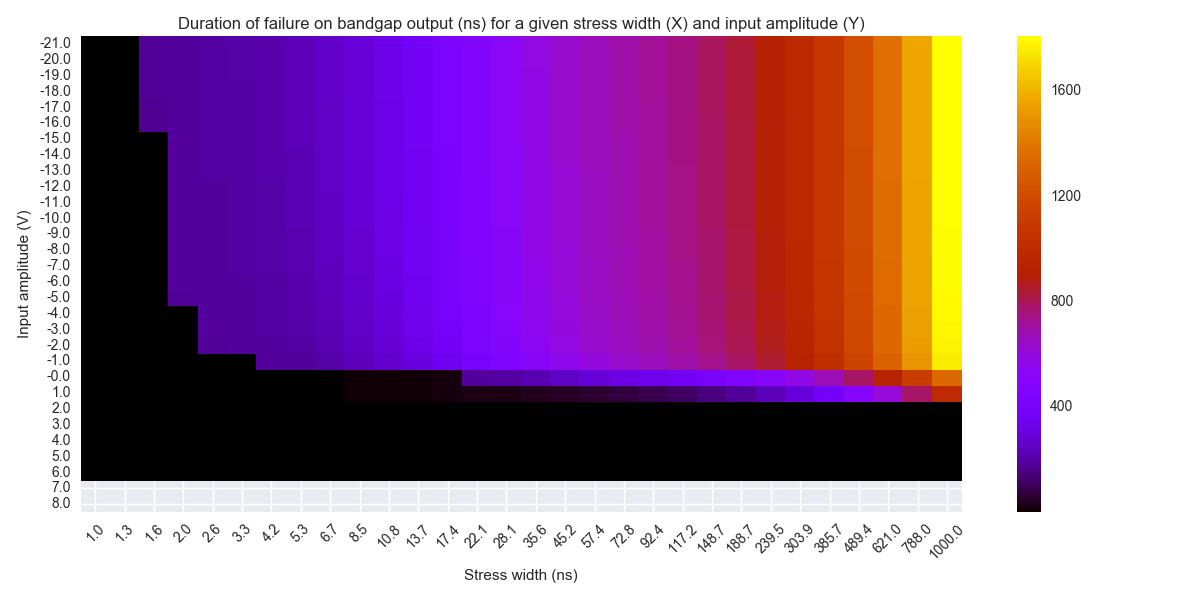
\includegraphics[width=\textwidth]{src/4/figures/bandgap_cz.png}
  \caption{Bandgap characterization}
  \label{bandgap_wb}
\end{figure}

\begin{figure}[!htbp]
  \centering
  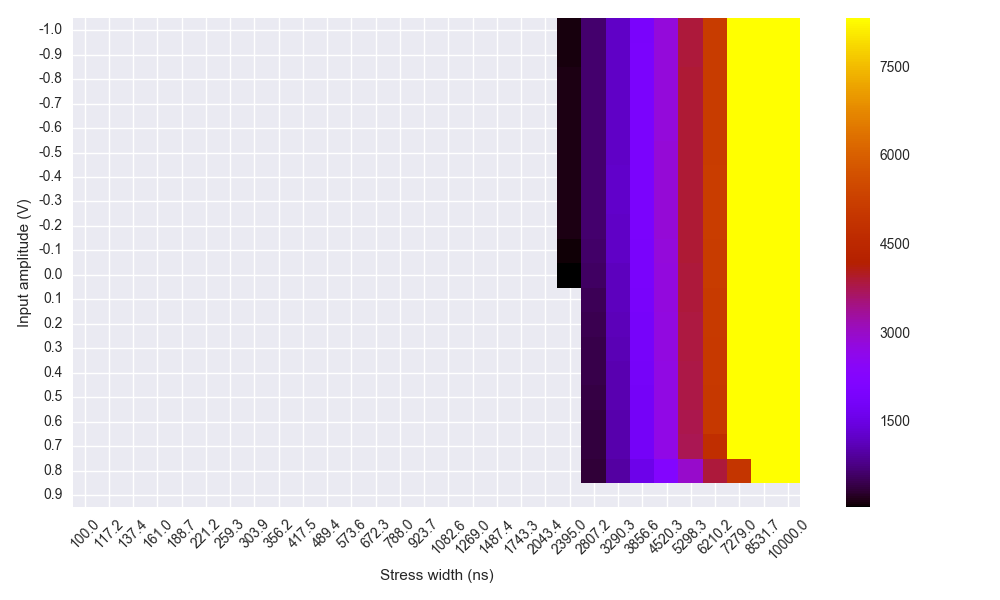
\includegraphics[width=\textwidth]{src/4/figures/regulator_cz.png}
  \caption{Regulator characterization}
  \label{regu_wb}
\end{figure}


% Characterization done, now perform chaining
After the characterization phase, it is now possible to chain the models together to evaluate the entire function's robustness, using method described in \label{sec:block-chaining}.
To check the validity of the model, a rectangular pulse is injected on the global input (pre-regulator input).
The chain of models is used to predict, without running any more simulations, the failure or not on the output pin.
For the purpose of this test, the input stress will be generated by a \gls{tlp} generator, producing a pulse of 100ns duration and -50V amplitude.

% Do it on one pulse config
First, the coordinaates (100ns, -50V) are reported on curve \ref{pre_regu_wb}, the first block model of the system.
%TODO: PAS POSSIBLE, CAR COURBES MONTRENT DC + STRESS
This point indicates a failure on the output of the pre-regulator, for a duration between XXns and XXns.
This gives the next point coordinates (XXns, -XXV).
This point is reported on the bandgap's model, the next block in the system.
Using these coordinates in the curve \ref{bandgap_wb} indicates a failure on the bandgap output between XXns and XXXns.
Finally, the point corresponding to the best-case output of the bandgap (XXXns, -XXV) is used as an input for the final block.
This gives a failure on the final output comprised between XXXns and XXXX ns.
In conclusion, the model chain estimated that for a -50V 100ns stress on the input, the regulation function will be at fault (output < XXV) for more than XXXX ns.

%TODO: SHOW ALL THREE CZ CURVES WITH POINT REPORT FROM ONE TO ANOTHER

% Perform standard complete simulation for reference
This result is then tested against a complete simulation of the entire regulation function (all three block).
The simulation circuit is given Fig. X.
This simulation uses transistor-level models, and will serve as a reference to compare the model-chain against it.
The same (100ns, -50V) rectangular pulse will be injected on the global input, and the global output will be monitored as well.
To check the validity of the model, we also monitor intermediate voltages, at the output of the pre-regulator and the bandgap.
The simulation of the input, pre-regulator output, bandgap output and final (regulator) output are given fig. X.

%TODO: SCHEMATIC FULL CIRCUIT

%TODO: PLOT TRANSIENT SIMULATIONS, USING 2 * 2 GRID, PLOTTING INPUT, PRE_REG_OUT, BANDGAP_OUT and REGU_OUT

% Result of the simulation
The simulation showed that for the given stress, the output will go below XXV for XXXns.
There is a rather large difference with the model chain.
To try to explain this difference, intermediates nodes are monitored.

% Error at the first block
The output of the pre-regulator is below X V (failure criteria) for XX ns in the full simulation while the model predicted XX ns.
Already, at this first block, there is a large difference between the simulation and the model.

% Error at the second block
The output of the bandgap (second block) shows even a higher difference.
In simulation, the output goes below XX V for XXX ns, while the model predicted XXX ns.

% Conclusion regarding this first simulation
Not only each curve introduces an important error, but errors tend to accumulate after each block.

% Test further simulation vs model
To test further the model versus the reference simulation, a set of different stresses are injected, with different properties.
The goal is to test the model on a larger set of input stresses.
For each stress, the result predicted by the model and the result obtained by the reference simulation are compared.
Results are summarized in table \ref{tab:comparison-multiple-pulses}.
The entire process is summarized in fig. X.

\begin{table}[!htbp]
\centering
\begin{tabular}{@{}|c|c|c|c|@{}}
\toprule
\multicolumn{2}{|c|}{\begin{tabular}[c]{@{}c@{}}Stress\\ properties\end{tabular}} & \multicolumn{2}{c|}{Results} \\ \midrule
duration (ns)                           & amplitude (V)                           & Reference      & Model       \\ \midrule
1 ns                                    & -5V                                     & no fail        & no fail     \\ \midrule
1 ns                                    & -10V                                    &                &             \\ \midrule
1 ns                                    & -15V                                    &                &             \\ \midrule
10 ns                                   & -5V                                     & fail 10ns      &             \\ \midrule
10 ns                                   & -10V                                    &                &             \\ \midrule
10 ns                                   & -15V                                    &                &             \\ \midrule
50 ns                                   & -5V                                     &                &             \\ \midrule
50 ns                                   & -10V                                    &                &             \\ \midrule
50 ns                                   & -15V                                    &                &             \\ \midrule
500 ns                                  & -5V                                     &                &             \\ \midrule
500 ns                                  & -10V                                    &                &             \\ \midrule
500 ns                                  & -15V                                    &                &             \\ \bottomrule
\end{tabular}
\caption{Comparison between simulation and reference for several pulse configurations}
\label{tab:comparison-multiple-pulses}
\end{table}

% Conclusion regarding the tables, differences observed

%TODO Review next
% Where does error come from ? Load impedance
Previously, it was indicated that all WnB curves were extracted with a fixed Zout = 1M\textOmega.
When connected together, each block (pre-regulator, bandgap, regulator) sees a load impedance on its output much different than that.
Thus, it is important to evaluate the impact of this value on the Wunsch and Bell characterization curve.
The pre-regulator is characterized again, this time with a load impedance of 100\textOmega.
This value is rather small impedance, but sufficiently high to not draw too much current on the pre-regulator.
This second characterization is given fig. X.

%TODO: CHARACTERIZATION WITH Z LOW IMPEDANCE

This characterization is compared with the one extracted with 1M\textOmega\.
To make the comparison easier, curves for failure above 1ns, 10ns, 100 ns and 1us were plotted separately (see fig. X).
MAKE COMPARISON

%TODO: COMPARISON Z LOW IMPEDANCE Z HIGH IMPEDANCE 2 * 2 1n -> 1u

SO FAR, CONSIDERED IMPEDANCE AS STATIC AND REAL.
TALK ABOUT IMAGINARY IMPEDANCES, AND DYNAMIC IMPEDANCES

TALK ABOUT ERROR CAUSED BY GRADIENT ?
